%TODO kohrenz->resolution? wird nicht verwendet in auswertung


\documentclass[a4paper]{scrartcl}

\usepackage[utf8]{inputenc}
\usepackage[english]{babel}
\usepackage{lmodern} 
\usepackage[T1]{fontenc}
\usepackage{booktabs}
\usepackage{multirow}
\usepackage{wrapfig}


% PAKETE
\usepackage{siunitx}
\usepackage{graphicx}
\usepackage{placeins}
\usepackage{longtable}
\usepackage{enumitem}
\usepackage{bbm}
%\usepackage{sidecap}


\usepackage{amssymb} % math symbols
\usepackage{amsmath} % ams
\usepackage{amsfonts} % mathmatical fonts

% caption indenting
 \usepackage[format=plain,indention=0em,labelfont=bf,margin=1em]{caption} 
 \usepackage{subfig} %subfigures ^^
\usepackage[protrusion=true,expansion=true]{microtype} % denser font, "-" behind line
\usepackage{esint} % nicer double and triple integrals
\usepackage{fancyhdr} % fancy headers
\usepackage[colorlinks=true,linkcolor=black,citecolor=black,filecolor=black,urlcolor=black]{hyperref}



% EINSTELLUNGEN
\sisetup{seperr,repeatunits=false}
\numberwithin{equation}{section}
\numberwithin{figure}{section}
\numberwithin{table}{section}

% EIGENE FUNKTIONEN
\newcommand{\re}{\operatorname{Re}}
\newcommand{\im}{\operatorname{Im}}
\newcommand{\gquote}[1]{\glqq #1 \grqq}

\newcommand{\eq}[2]{\begin{equation}#1\label{#2}\end{equation}}
\newcommand{\eqand}[0]{\hspace{.25cm} \bigwedge \hspace{.25cm}}
\newcommand{\grafik}[2]{\begin{figure}[h]\centering \includegraphics[width=10cm]{#1.eps}  \caption{#2} \label{#1} \end{figure} }
\newcommand{\grafikq}[3]{\begin{figure}[h]\centering \includegraphics[width=10cm]{#1.eps}  \caption[#2]{#3} \label{#1} \end{figure} }
\newcommand{\tbl}[3]{\begin{table}[h]\caption{#1}\label{#2}\begin{center}#3\end{center}\end{table}}
\newcommand{\Abbildung}[1]{\textsl{Abbildung \ref{#1}}}
\newcommand{\AbbildungI}[1]{\textsl{(Abbildung \ref{#1})}}
\newcommand{\Tabelle}[1]{\textsl{Tabelle \ref{#1}}}
\newcommand{\TabelleI}[1]{\textsl{(Tabelle \ref{#1})}}
\newcommand{\Formel}[1]{(\ref{#1})}
\renewcommand{\d}{\mathrm{d}}
\newcommand{\ve}[1]{\mathbf{ #1} }

\title{Ma 6: Atomic Force Microscopy (AFM)}
\subtitle{Tutor: Ch. Lotze}
\author{Benjamin Huber, Carolin Wille}
\date{January 2, 2012}

\begin{document}
\thispagestyle{empty}
\maketitle
\tableofcontents
\clearpage


\section{Introduction}
Atomic Force Microscopy (AFM) is a surface imaging technique, which has a very high resolution on the order of nanometers. It was developed in 1986 by Binnig, Quate and Gerber subsequently of the invention of the scanning tunneling microscope (STM) in 1981. STM, which uses the quantum mechanical tunneling current between the tip of the microscope and the sample to investigate the topography of a surface, requires conducting samples. In contrast, the AFM technique is based on very general forces, like the van-der-Waals force or chemical forces and thus allows studies of conducting as well as of non-conducting materials.

The AFM measures the forces along the sample's surface with a cantilever, on which a sharp tip is mounted. The forces influence the cantilever by either bending it towards or away from the surface. The tilting or even shearing of the cantilever is detected by a laser beam, which is reflected from the cantilever's backside towards a photo-diode. The AFM is equipped with an electronic feed-back regulation circuit, such that the distance between the tip and the sample can be held constant, which is used in some operation modus. The AFM is mounted on a piezo-element, with which the movement within the sample plane and the height can be controlled. Usually the tip moves forward line-wise like a common printer, but it always scans the lines moving in the same direction.

\begin{figure} 
 \centering
\subfloat[][Schematic Picture of an AFM]
{         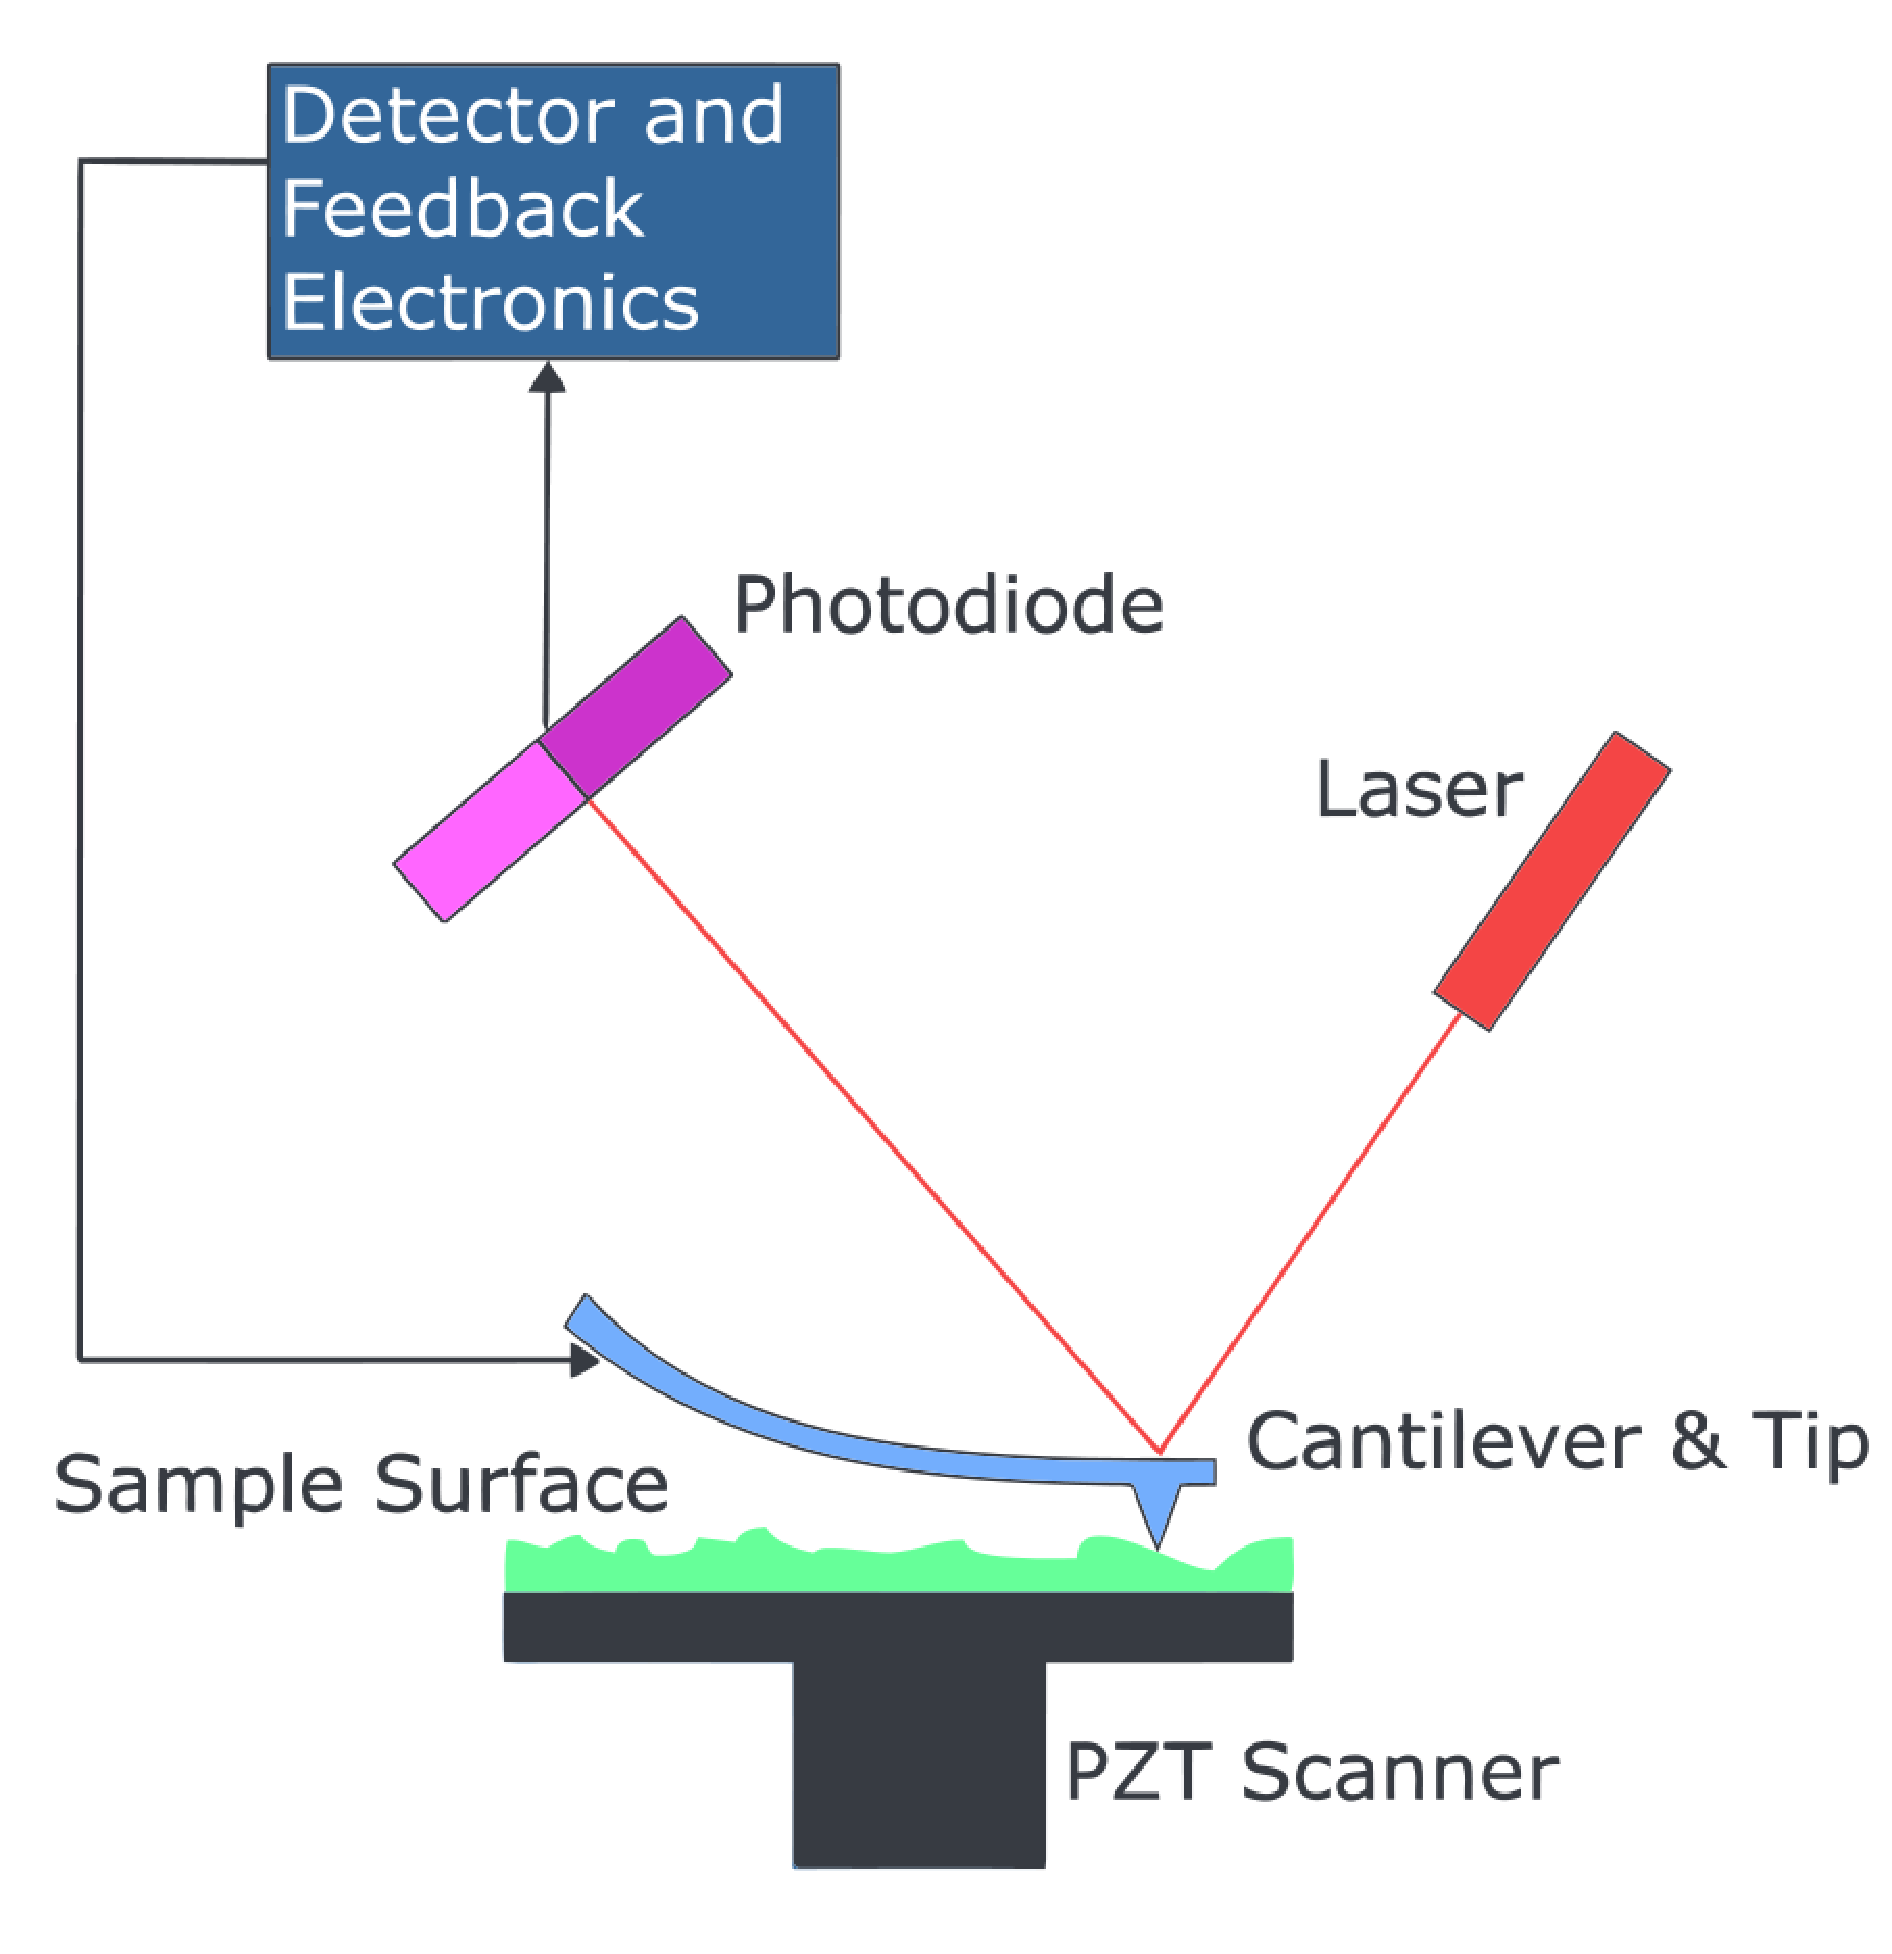
\includegraphics[width=0.45\linewidth]{img/afmsetup.pdf}       
}
 \hfill
\subfloat[][Scanning Process]
         {}%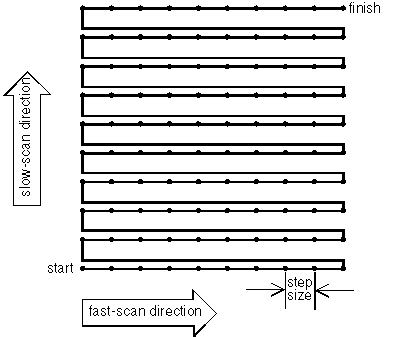
\includegraphics[width=0.45\linewidth]{img/scan.png}}
\caption{
\small  \textbf{(a)} Typical AFM Set-Up and \textbf{(b)} scanning directions, Sources: \url{http://en.wikipedia.org/wiki/Atomic-Force-Microscope}, \cite{book}  } 
	\label{fig:setup}
\end{figure}



\subsection{Relevant Forces acting on the AFM}
The forces acting on the AFM tip can be divided into chemical, electric, magnetic and van der Waals force
\eq{F_\text{tot}=F_\text{ch}+F_\text{el}+F_\text{mag}+F_\text{vdW} \; .} {forces}
The chemical force and the van der Waals force $F_\text{ch}$ and $F_\text{vdW}$ can be modelled by the empirical Lennard-Jones potential
\eq{V_\text{LJ}=4\epsilon\left[\left(\frac{\sigma_{0}}{r}\right)^{12}-\left(\frac{\sigma_{0}}{r}\right)^{6}\right] \; , }{jones}
where the first term describes a strong, but short ranged repulsion due to the Paul-principle acting on the overlapping electron clouds of the smaple and the tip, while the second term describes the attraction through the van der Waals force, the attraction between non-permanent dipoles in atoms. The van der Waals force acting on the tip, can be approximated by the force of a plane surface on a sphere of radius $R$ at a distance $d$ 
\begin{equation}
F_\text{vdW}=\frac{HR}{6d^{2}} \; ,
\end{equation}
$H$ is the Hamaker constant, depending on the tip-sample-combination via the atom density of both. 

The electric or Coulomb force $F_\text{el}$ can be understood in terms of a capacitor, that is formed by the tip and the sample. The voltage between the two poles is given by the contact potential
\begin{equation}
U_{contact}=\frac{1}{e}\left(\Phi_{tip}-\Phi_{sample}\right),
\end{equation}
where the $\Phi_i$ are the work functions of the respective materials. If an additional bias voltage is applied the total voltage is $U=U_\text{bias}+U_\text{contact}$ and the electric force is given by the spatial derivative of the potential 
\begin{equation}
F_\text{el}=\frac{\partial }{\partial z} \tfrac 1 2 C U^2 = \frac{1}{2} \frac{\partial C}{\partial z} (U_\text{bias}+U_\text{contact})^2 \; , \label{eq:elec}
\end{equation}
where $C$ is the capacity.

The magnetic force $F_{mag}$ is only relevant for magnetized tips and magnetic samples and is therefore not discussed here. 

\begin{figure} 
 \centering
\subfloat[][Force between tip and sample]
         {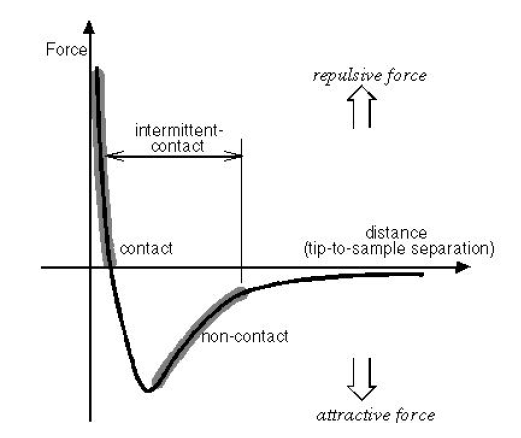
\includegraphics[width=0.6\linewidth]{img/forces.png}}
\caption{
\small \textbf{(a)} Force acting on the AFM tip vs tip-sample distance. Different distances and the corresponding signs of the force (repulsive/attractive) are used in the two different operation modi (contact/non-contact).
Source: \url{http://en.wikipedia.org/wiki/Magneto-optic_Kerr_effect}. } 
	\label{fig:forces}
\end{figure}

\subsection{Operation Modes}  
\subsubsection*{Contact Mode}
With the typical set-up and acting forces described in the previous section, it is possible to select different operation modi of the AFM. The simplest one is the \textbf{contact mode}, where the distance between tip and sample is so small, that the repulsive Pauli force dominates. Contact mode can be used in two ways, either the height of the AFM tip is kept constant and the changes of the cantilever deflection is recorded yielding a force-profile of the surface, or the force is kept constant via regulating the height of the tip using the feed-back electronics. Thus, a height profile can be generated. However, as the distance between tip ans sample is very small in both cases, the risk of damaging both tip and sample is a big disadvantage of this modus. 
\subsubsection*{Non-Contact Mode}
This problem can be avoided in \textbf{non-contact} mode, where the tip-sample distance is in the attractive force regime. To avoid spontaneous crashes into the sample in regions with high attractive forces, the cantilever is made of sufficiently hard materials. In non-contact mode the cantilever is not gliding statically over the sample surface, but is driven to oscillate at a frequency close to its own resonance. The distance between tip and sample is related to the magnitude of the attractive force, which influences the resonance curve of the cantilever oscillation. If the oscillation frequency and amplitude are held constant, the tip-sample distance has to regulated via the height of the tip. In this way, the topography  of the sample can be scanned. In more detail, the equation of motion of the tip-sample distance can be modeled as a damped, driven harmonic oscillator with an additional attractive force $F_a$
\begin{equation}
m\ddot{z}+\gamma \dot{z}+kz=F_{0} \exp( {i \Omega t})+F_{a} \label{eq:differential}
\end{equation}
where $z$ is the oscillation amplitude around equilibrium position, $m$ is the mass, $\gamma$ is the damping factor, $k$ is the spring constant , $F_0$  the amplitude and $\Omega$ the frequency of the driving force. The oscillation frequency is given by $\omega_0\,=\,\sqrt{k/m}$. If the oscillation amplitude is small, it is reasonable to expand the attractive force in powers of the oscillation amplitude. The constant term leads to a shift of the equilibrium position and is not important. The linear term can be included into an effective spring constant
\begin{equation}
k_\text{eff}=k-\frac{\partial F_{a}}{\partial z} \label{eq:change}.
\end{equation}
This shift corresponds to a shift of the resonance frequency 
\eq{\Delta \omega_0 = -\frac{\omega_0}{2 k} \frac{\partial F_a}{\partial z} }{shift}
and therefore can be connected to a change of the oscillation amplitude $A$, which is given by \cite{martin}
\begin{equation}
A=\frac{ A_0 \omega_0 / \Omega  }  { \sqrt{1 + Q^2(\Omega / \omega_0 - \omega_0 / \Omega )^2 }  } ,
\end{equation}
where $A_0=F_0/m$ is the amplitude of the oscillator without driving force and $Q=\omega_0/2\gamma$ is the quality factor of the cantilever. With eq. \Formel{shift} the force gradient can be expressed in terms of the quality factor and the amplitude ratio $a=A_0/A$
\begin{equation}
\frac{\partial F_{a}}{\partial z}=k\left(\frac{1-2a^{2}+\sqrt{4Q^{2}\left(a^{2}-1\right)+1}}{2\left(Q^{2}-a^{2}\right)}\right) \; .
\end{equation}

\subsubsection*{Electronic Properties and Tip Geometry}
In order to study the contact potential $V_C$ between tip and sample, one can measure the force with respect to the applied voltage. Relation \Formel{eq:elec} states, that the electrical force hast a minimum at $V_\text{bias} = -V_C$. Thus, $V_C$ can be measured via the force, e.g. the direct bending of the cantilever ore a change in the oscillation amplitude. Alternatively the height-regulation of the afm can be used to measure the distance vs the voltage. Also in this case, the minimum of the curve gives the contact potential, however the derivative of the capacitance with respect to the distance $\frac{\partial C}{\partial z}$ varies with the distance. This variation depends on the tip-geometry and has been classified by L. Olsson et al. \cite{olsson}. Therefore, the distance-voltage curves in constant force (or better force-gradient) mode can be used to do some estimates about the tip geometry.

\begin{figure} 
 \centering
      % 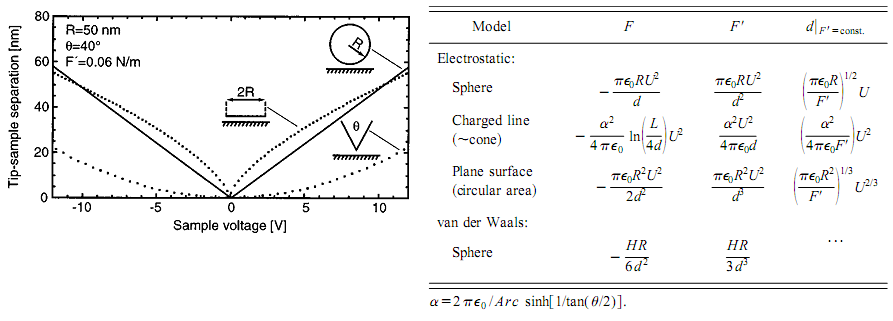
\includegraphics[width=\linewidth]{img/tip.png}
\caption{
\small \textbf{Left:} Different Distance-Voltage Curves (const. force gradient) for different sample geometries. \textbf{Right:} Analytical expressions for force $F$ , force gradient $F'$ and distance $d$ at constant force for different tip geometries. Source: Olsson et al. \cite{olsson} } 
	\label{fig:geometry}
\end{figure}

% \subsection{Systematic Errors and Artifacts}



\section{Analysis}

\subsection{Topographies}
\begin{figure} [p]
 \centering
 \begin{tabular}{l r}
 \subfloat[][Sample A $5\times5\mu m^2$]
{         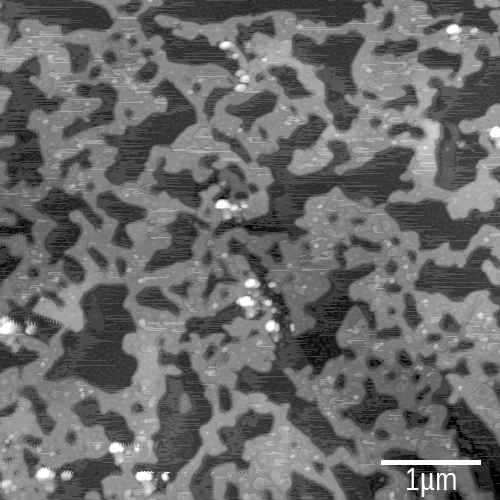
\includegraphics[width=0.37\linewidth]{img/AuG.jpg}       }
&
\subfloat[][Sample A $1\times1\mu m^2$]
         {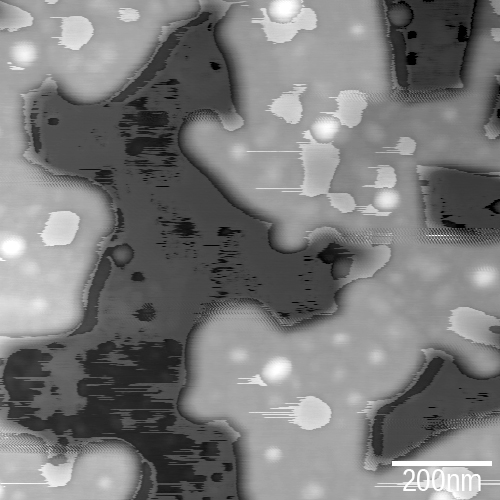
\includegraphics[width=0.37\linewidth]{img/AuGMacro2.jpg}}
\\
\subfloat[][Sample B $4\times4\mu m^2$]
{         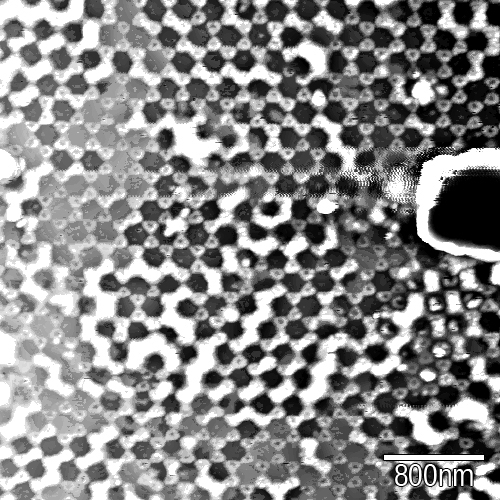
\includegraphics[width=0.37\linewidth]{img/balls.jpg}       }
&
\subfloat[][Sample B $1\times1\mu m^2$]
         {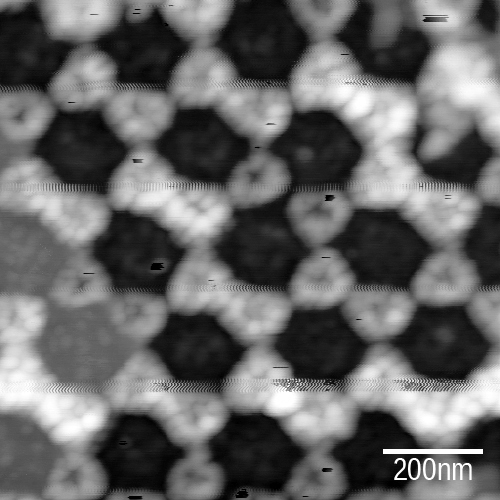
\includegraphics[width=0.37\linewidth]{img/ballsMacro.jpg}}
\\
\multicolumn{2}{c}{
\subfloat[][Fourier transform of Sample B with close-up]
         {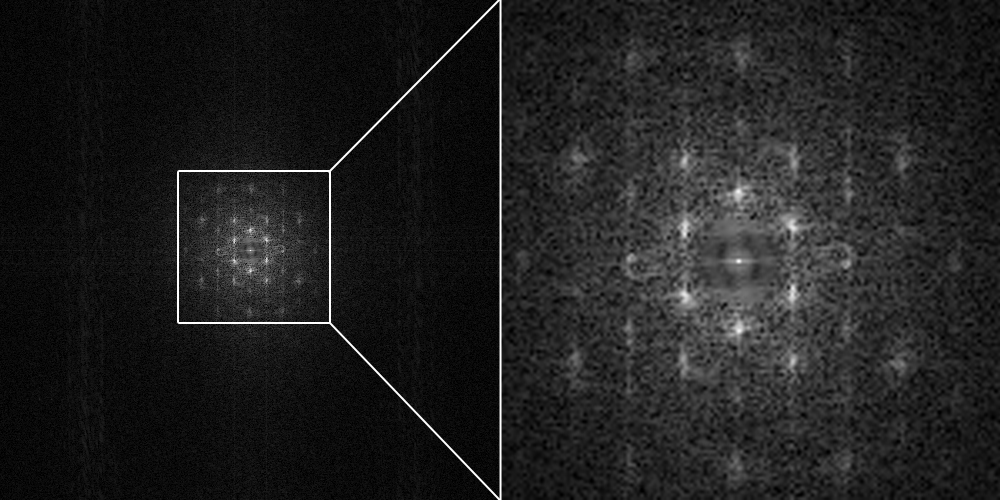
\includegraphics[width=0.8\linewidth]{img/fft.jpg}}
}
 \end{tabular}
\caption{
\small  \textbf{(a)-(c)} Topographies of samples A and B with different resolutions. \textbf{(d)} Topography of Sample B, measurement of the length of the rows of holes resulted in diameters (in nm, from top to bottom) $238\pm6, 255\pm9, 248\pm5, 246\pm5, 247\pm5$. \textbf{(e)} Fourier transform of (c). Contrast edited to highlight the peaks in the spectrum.
 } 
	\label{fig:topo}
\end{figure}
Point by point two samples were scanned with different resolutions, revealing their surface structure. The first sample consists of a thin layer of gold evaporated on a graphite substrate. The unordered surface that this process generates can be seen in pictures \ref{fig:topo}a and \ref{fig:topo}b. Because the measurement was done in the dynamic mode and the sample was not put in a vacuum, water droplets pollute the picture.  

The second sample suffers from these droplets as well. Especially well visible in \ref{fig:topo}c. For the higher resolution picture \ref{fig:topo}d on the other hand it was possible to choose a very clean region. The periodic pattern was created by polysterene balls. After evaporating the gold an the sample, these balls were removed with a tape, leaving behind a periodic pattern of holes that naturally resembles a sphere packing.

A closer investigation of these pictures quickly gives an estimate of the diameter of the used spheres. Looking only at the fast scanning direction (left to right in the pictures) and measuring over as many balls as possible in picture \ref{fig:topo}d gives a mean diameter of $(246.3\pm6.0)\,\text{nm}$ where the error is mainly due to the variance of the data.

To manage the large amount of data of picture \ref{fig:topo}c another method was used. To use all of the topography at once, a Fourier transformation was performed. Strong periodic elements corresponding e.g. to the distance between two balls from left to right can be found all over the picture and thus create a strong peak in the Fourier transformed amplitude plot. With changed contrast settings to better highlight the peaks, such an amplitude plot can be found in \ref{fig:topo}e. The 34 peaks that can be found on it correspond to 17 standing waves, each giving an independent measurement of the ball diameter.

Again the drift has to be considered. It causes the fast scanning direction to be more precise and may compress or stretch the slow scanning direction. To account for this, the direction of the standing waves was noted as well and instead of a constant radius in all direction, an elliptical model was fitted (see figure \ref{fig:diameterfit}). The final value for the diameter in the fast direction using this method is $(242.3\pm 2.6)\,\text{nm}$. From the diameter in the slow direction the amount of compression due to thermal drift can be approximated to be $(7.1\pm1.7)\%$ compared to the fast direction.

\begin{figure}
\centering
	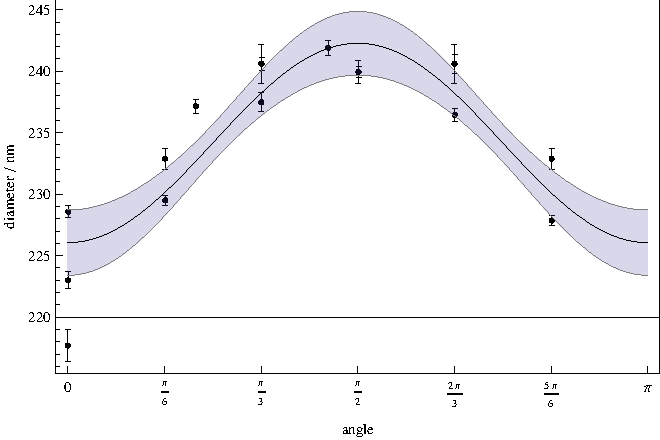
\includegraphics[width=0.8\linewidth]{img/diameterfit.pdf}
	\caption{\small An elliptical model fitted to the measured diameter in dependence on the angle. The angle $\pi/2$ corresponds to the fast scanning direction. The two diameters in fast and slow direction resulting from this fit are $(242.3\pm2.6)\,\text{nm}$ and $(226.1\pm2.7)\,\text{nm}$. To indicate the quality of the fit, the 95\% confidence intervals are plotted in gray. }
	\label{fig:diameterfit}
\end{figure}



\section{Summary and Discussion}
Using an atomic force microscope, two samples were investigated. Their topography was determined and voltage spectroscopy was used to investigate the contact potentials of graphite and gold and make statements about the form of the tip.

The recording of topography was very successful and revealed the surface structure of both samples on the one hand and allowed for very precise determination of the ball diameter on the other hand. Using all the data in a $4\mu m \times 4\mu m$ scan via a Fourier transformation lead to the value of $(242\pm 3)\,\text{nm}$ for the diameter and a compression of the slow scanning direction of $(7\pm2)\%$ compared to the fast direction.

The voltage spectroscopy turned out to be much more problematic. Due to the high number of water droplets a lot of measurements had to be discarded. 
%hmm kann das noch nicht wirklich schreiben ohne deine ergebnsse zu kennen ^^


\clearpage
 \bibliographystyle{unsrt}
\bibliography{bib}

\end{document}


